
\chapter{Classification: concepts}

\section{Labeled and unlabeled examples}

\index{classification}
\index{classifier}
\index{label}
\index{unlabeled examples}
\index{labeled examples}
\index{examples, labeled and unlabeled}
\index{input!to a classifier}
\index{output!of a classifier}

In the activity of classification, the \textbf{target} variable we aim to
predict is categorical. We sometimes also call this variable the
\textbf{label}. Since this is a \textit{supervised} process, we are provided
with example objects of study that have known ``true answers.'' These are
called \textbf{labeled examples}. The goal of the activity is to produce good
predictions of the labels for other, \textbf{unlabeled examples}. A program
that can make such predictions, after having studied the labeled examples, is
called a \textbf{classifier}.

\index{feature}
\index{attribute}

The predicted label can be seen as the ``output'' from our classifier. All of
the other variables are essentially the inputs to our process, which we use to
make our predictions. These variables are called \textbf{features} (or
sometimes, \textbf{attributes}).

In terms of Pandas data structures, all these labeled examples will normally
come packaged in a \texttt{DataFrame}. Each row of the \texttt{DataFrame} will
be one labeled example, with its features as columns and its target/label as a
column (traditionally, the rightmost one).

This is illustrated in Figure~\ref{fig:labeledTrainTest}. Here we have some
labeled examples for a data set on NFL fans. Each row represents one fan, and
shows various features of their existence -- how old they are, where they were
born, where they live now, and how many years they've lived in their current
residence. The rightmost column gives the target: the team to whom this fan has
sworn their allegiance. Our aim would be to predict which team a fan might root
for, based on what we know about them. Lest you think this example is
frivolous, consider that a sporting goods company might want to send catalogs
(paper or electronic) to potential customers, and it would probably boost sales
if the cover image of the catalog featured a model wearing apparel from
the customer's favorite team, rather than their rival.

\begin{figure}[ht]
\centering
\fbox{
\mbox{
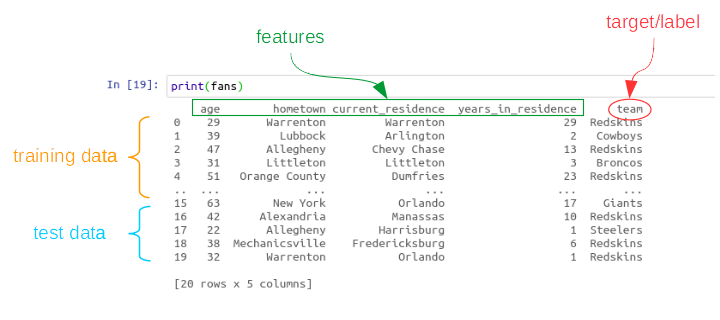
\includegraphics[width=1.05\textwidth]{footballML.png}
}}
\smallskip
\caption{Some labeled examples, divided into training and test sets.}
\label{fig:labeledTrainTest}
\end{figure}

\index{training data}
\index{test data}

You'll also see in the figure that I've split the rows up into two groups. The
first group is called the \textbf{training data}, and the second, the
\textbf{test data}. (Normally we'll shuffle all the rows before assigning them,
so that we don't put all the top rows of the \texttt{DataFrame} in the training
set and all the bottom ones in the test set. But that's harder to show in a
picture.)

\section{Three kinds of examples}

Now here's the deal. There are \textit{three} kinds of example rows we're going
to deal with:

\begin{compactenum}
\item \textbf{training data} -- \textit{labeled} examples which we will show to
our classifier, and from which it will try to find useful patterns to make
future predictions.
\item \textbf{test data} -- \textit{labeled} examples which we will
\textit{not} show to
our classifier, but which we will use to measure how well it performs.
\item \textbf{new data} -- \textit{unlabeled} examples that we will get in the
future, after we've deployed our classifier in the field, and which we will
feed to our classifier to make predictions.
\end{compactenum}

The purpose of the first group is to give the classifier useful information so
it can intelligently classify.

The purpose of the second group is \textit{to assess how good the classifier's
predictions are.} Since the test set consists of labeled examples, we know the
``true answer'' for each one. So we can feed each of these test points to the
classifier, look at its prediction, compare it to the true answer, and judge
whether or not the classifier got it right. Assessing its accuracy is usually
just a matter of computing the percentage of how many test points it got right.

The third group exists because after we've built and evaluated our classifier,
we actually want to put it into action! These are new data points (new sporting
goods customers, say) for which we don't know the ``true answer'' but want to
predict it so we can send catalogs likely to be well-received.

\subsection{Thou shalt not reuse}

Now one common question -- which leads to a \textit{super} important point --
is this: why can't we use \textit{all} the labeled examples as training data?
After all, if we have 1000 labeled examples we've had to work hard (or pay
\$\$) to get, it seems silly to only use some of them to train our classifier.
Shouldn't we want to give it all the labeled data possible, so it can learn the
maximum amount before predicting?

The first reply is: ``but then we wouldn't have any test data, and so we
wouldn't know how good our classifier \textit{was} before putting it out in the
field.'' Clearly, before we base major business decisions on the results of our
automated predictor, we need to have some idea of how accurate its predictions
are.

It's then commonly countered: ``well, sure, but why not then re-use those data
points for testing? Instead of splitting the 1000 examples into training points
and test points, why not just use all 1000 for training, and then test the
classifier on all 1000 points? What's not to like?''

This is where the super important point comes in, and it's so important that
I'll put it all in boldface. It turns out that \textbf{you absolutely
\textit{cannot} test your classifier on data points that you gave it to train
on, because you will get an overly optimistic estimate of how good your
classifier actually is.}

Here's an analogy to make this point more clear. Suppose there's a final exam
coming up in your class, and your professor distributes a ``sample exam'' a
week before exam day for you to study from. This is a reasonable thing to do.
As long as the questions on the sample exam are of the same type and difficulty
as the ones that will appear on the actual final, you'll learn lots about what
the professor expects you to know from taking the sample exam. And you'll
probably increase your actual exam score, since this will help you master
exactly the right material.

But suppose the professor uses the \textit{exact same} exam for both the sample
exam and the actual final exam? Sure, the students would be ecstatic, but
that's not the point. The point is: \textit{in this case, students wouldn't
even have to learn the material.} They could simply memorize the answers! And
after they all get their A's back, they might be tempted to think they're
really great at chemistry...but they probably aren't. They're probably just
really great at memorizing and regurgitating.

Going from ``the kinds of questions you may be asked'' to ``\textit{exactly}
the questions you \textit{will} be asked'' makes all the difference. And if you
just studied the sample exam by memorization, and were then asked (surprise!)
to demonstrate your understanding of the material on a \textit{new} exam, you'd
probably suck it up.

\index{generalizing (to new data)}

And so, the absolute iron-clad rule is this: \textbf{any data that is given to
the classifier to learn from must \textit{not} be used to test it.} The test
data must be comprised of representative, but different, examples. It's the
only way to assess how well the classifier \textbf{generalizes} to new data
that it hasn't yet seen (which, of course, is the whole point).


